

\subsection{RQ-1: Effectiveness Comparison}
\label{sec:rq1}



\noindent\textbf{Experimental Design.} To investigate whether \toolname outperforms existing methods on repository-aware code translation tasks, we conducted comprehensive experiments on our constructed dataset. For each source function in the dataset, we performed translation using four distinct methods and determined whether the translated function succeeded by executing the project's test cases. We uniformly employed the DeepSeek V3 model for code translation and maintained consistent model parameters across all methods to eliminate confounding factors. Finally, we assessed the effectiveness of each method using compile rate and pass rate as evaluation metrics.

\noindent\textbf{Results.} The experimental results encompass four components: Overall Results, Statistics of Error Types, Comparison with Baselines, and Case Study.

\paragraph{Overall Results} Table~\ref{tab:rq1_combined} presents the compile rate and pass rate achieved when employing the DeepSeek V3 model. \toolname and the three baseline approaches were evaluated on our dataset for bidirectional translation between Java and C\#. For the 627 functions translated from C\# to Java, our method successfully compiled 363 functions and 299 functions passed all test cases. For the 655 functions translated from Java to C\#, 306 functions were successfully compiled and 245 functions passed all test cases.

\paragraph{Statistics of Error Types} For functions that failed to pass all test cases, we extracted the error logs and systematically categorized the error types. The results are presented in Table~\ref{locationTypeResults}. 

The predominant errors were compilation errors, with the most frequent issue being ``symbol not found''. 
This typically occurs when classes, methods, or fields defined in the source repository are absent in the target repository. This observation underscores that implementation differences between source and target repositories constitute the primary cause of translation failures, thereby emphasizing the critical importance of context collection in repository-aware code translation.

\begin{table}[!htbp]
\centering
\small
\caption{The error types of the functions that failed to be translated.}
\label{locationTypeResults}
\begin{tabular}{lcccc} 
\toprule
Error type    & C\# to Java / Java to C\#   \\ 
\midrule
Compilation Errors    & 264/349             \\ 
Runtime Errors   & 26/19                  \\ 
Functional Errors     & 36/41                   \\ 
Non-terminating Execution & 2/1             \\
\bottomrule
\end{tabular}
\end{table}


\textbf{\begin{figure}[htbp]
\centerline{
\includegraphics[width=1\linewidth]{figs/example.pdf}}
\caption{An example of a function translation using tools by \toolname}
\label{fig:example}
\end{figure}}


\paragraph{Comparison with Baselines} When compared with baseline approaches, \toolname achieves substantially higher compile and pass rates across both translation directions and all projects, although the magnitude of improvement varies. This demonstrates that \toolname exhibits excellent generalization capabilities across diverse projects and demonstrates strong robustness and adaptability. Notably, compared with direct code translation methods that do not incorporate agent-based approaches, our method shows substantial performance gains, confirming its effectiveness. In particular, \toolname achieves several-fold improvements in pass rate on the jgit and rocketmq-clients projects. For further analysis, taking the translation from C\# to Java as an example, Fig.~\ref{fig:venn} illustrates the overlap of successfully translated functions among different methods.



\begin{figure}[htbp]
\centerline{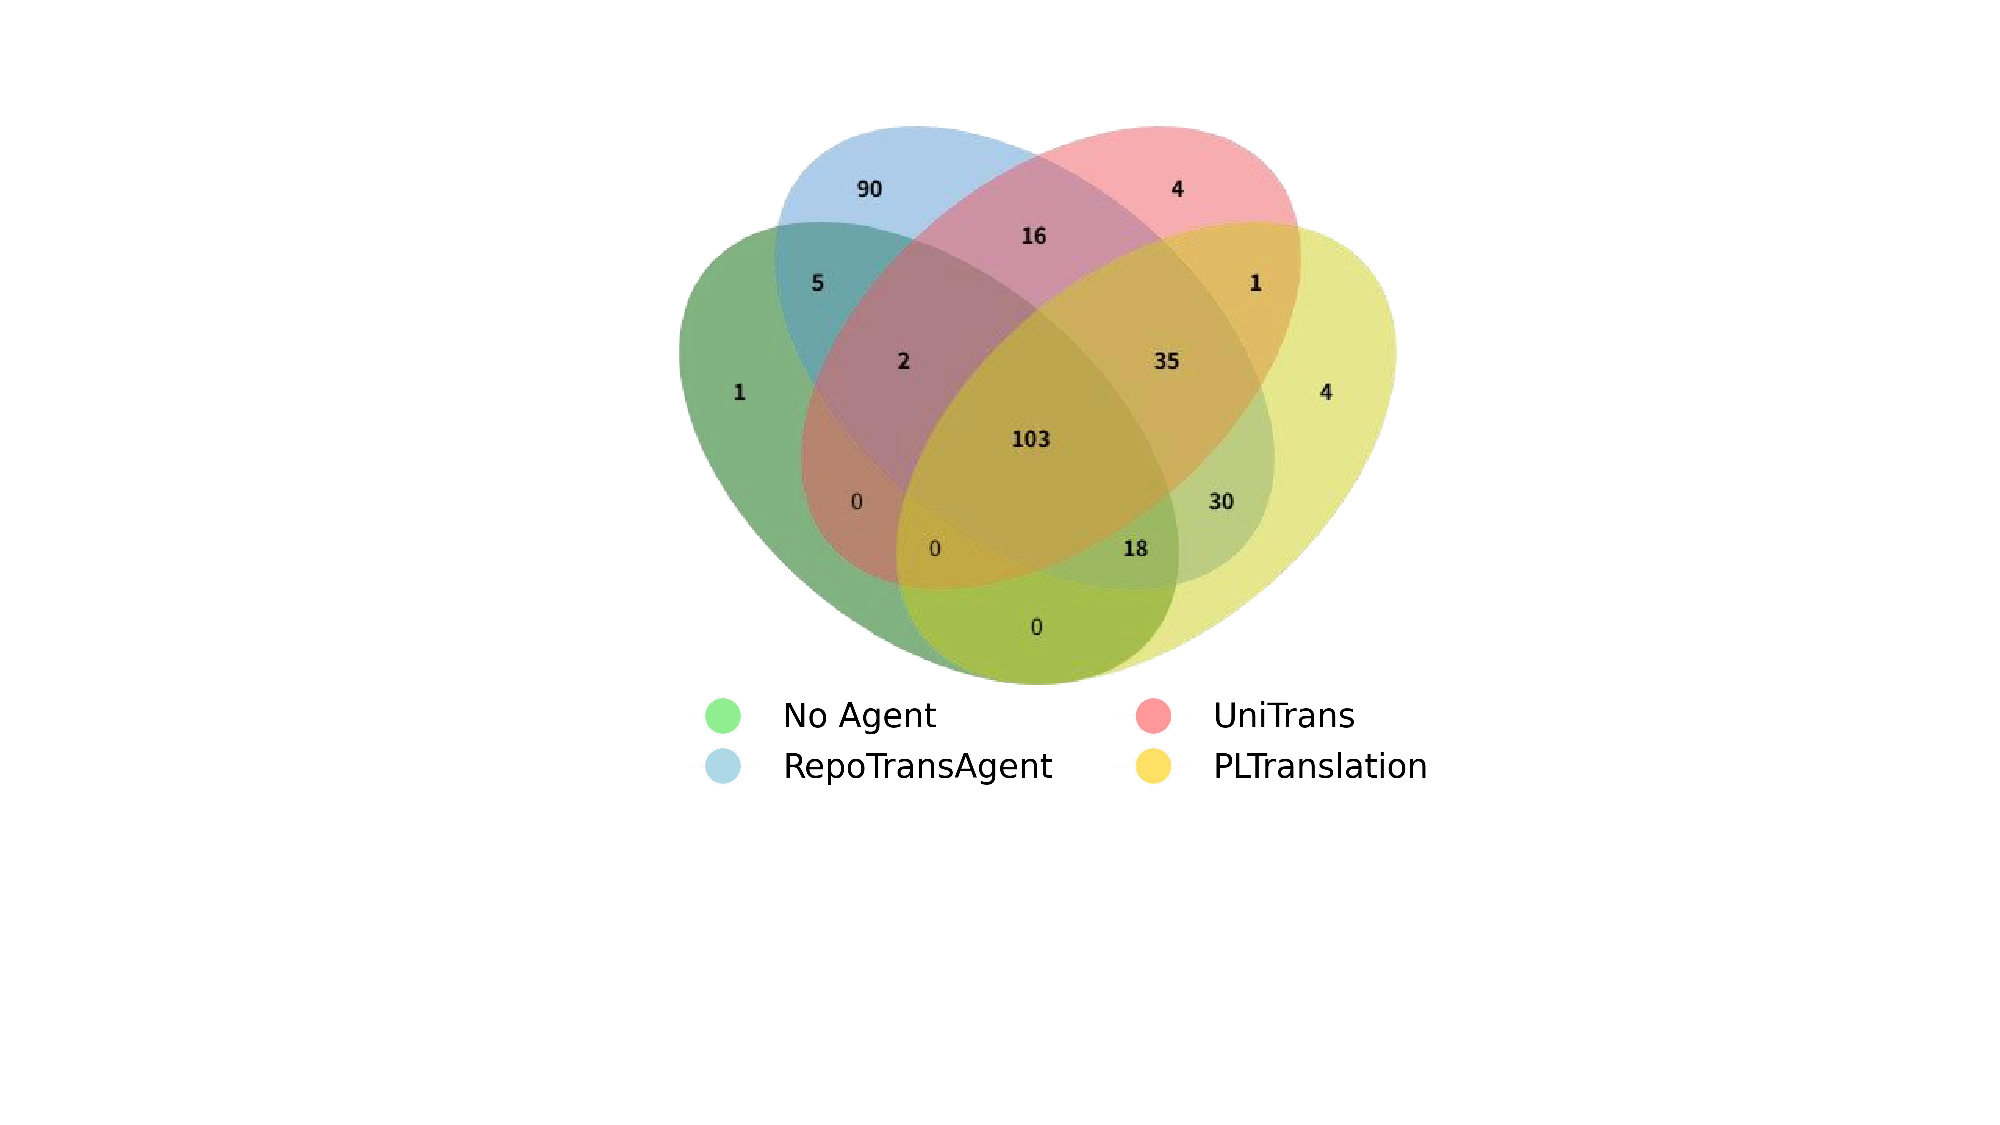
\includegraphics[width=0.6\linewidth]{figs/venn_1.pdf}}
\caption{The intersection of functions successfully translated by different methods}
\label{fig:venn}
\end{figure}


The results demonstrate that \toolname successfully translated nearly all functions that were handled by any of the three baseline methods, with only 10 functions successfully translated by at least one baseline but not by \toolname. Moreover, \toolname successfully translated 90 functions that none of the baseline methods managed to translate. We attribute this superior performance to \toolname's capability to effectively collect the most relevant context through collaborative coordination among different agents, and to iteratively correct errors during the translation process.

\paragraph{Case Study} Fig.~\ref{fig:example} presents a function that was successfully translated exclusively by \toolname. During the translation process, the agent first adhered to established guidelines, converting the C\# Dictionary data structure into Java's Map, and translating the C\# foreach loop into a Java for loop. Subsequently, the agent invoked the find\_target\_imports tool and discovered that the target file did not import the CellUtil enum, but instead imported the CellPropertyType enum. Consequently, the agent appropriately translated CellUtil into CellPropertyType.

Subsequently, by invoking the find\_target\_class\_info tool, the agent identified that the CellAddress class in the target repository did not contain the calculateCount method but did include a method named collectCount. Through semantic inference from the method name that the two methods were likely functionally equivalent, the agent replaced cell.CalculateCount with cell.collectCount in the translation.

Through these systematic steps, the agent successfully translated the source function. This example demonstrates the effectiveness of each tool function: the agent can selectively gather the context necessary for translating the source function and exhibits reasoning capabilities, enabling it to address challenges that static analysis cannot resolve.


\intuition{
{\bf Answer to RQ-1:}
\toolname significantly outperforms the baseline approaches in improving both compile and pass rates, with the average compile rate increasing from 26.07\%–30.47\% to 55.34\%, and the average pass rate rising from 18.59\%–28.16\% to 45.84\%. Furthermore, \toolname demonstrates consistent performance across various projects, exhibiting strong generalization capabilities.    
}




